\section{Resultados en Xschem, con los parámetros obtenidos \label{sec:s2}}

\begin{center}
	\begin{minipage}{12cm}
		\begin{tcolorbox}[title=Actividad 2]
			Utilizando el simulador NGSPICE en la herramienta de Xschem, simular el amplificador operacional con las razones $\frac{W}{L}$ calculadas previamente.
		\end{tcolorbox}	
	\end{minipage}
\end{center}

\begin{figure}[ht]
	\centering
	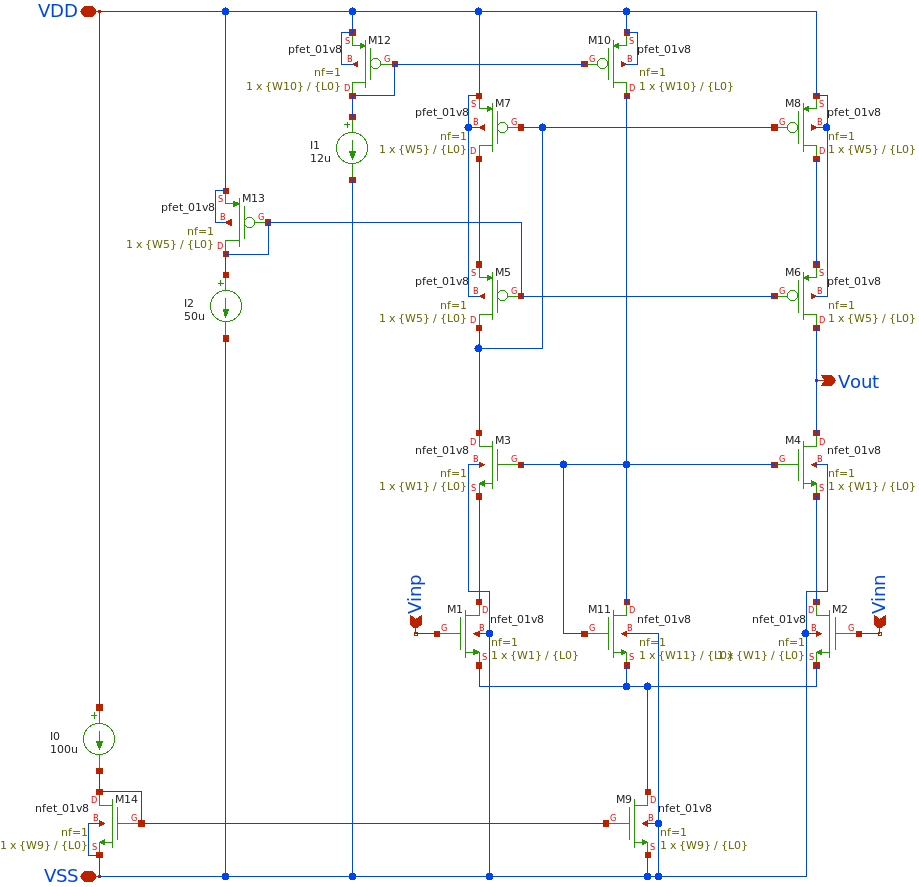
\includegraphics[scale=0.4]{CascodeOneStageOpAmp.png}
	\caption{Diagrama esquemático del amplificador operacional cascodo de una etapa. \label{fig:CascodeOneStageOpAmp}}
\end{figure}

\begin{figure}[ht]
	\centering
	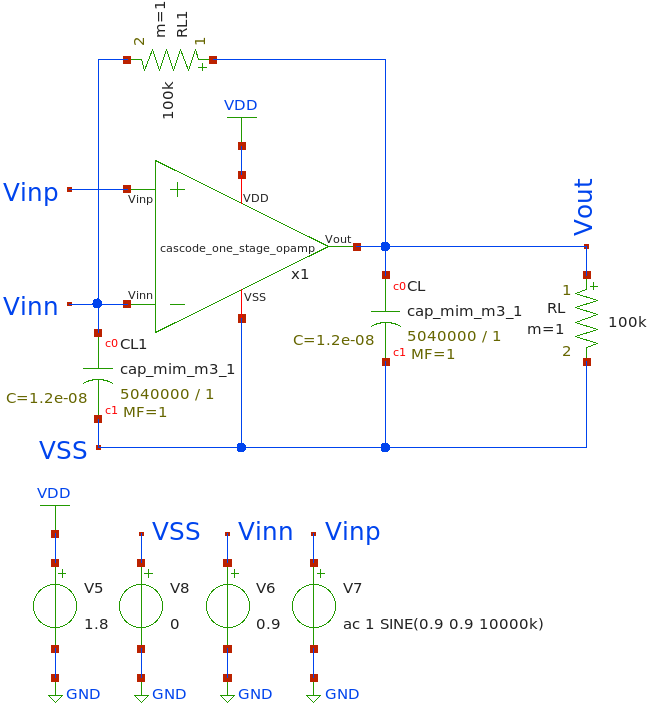
\includegraphics[scale=0.32]{CascodeOneStageOpAmpAv.png}
	\caption{Circuito utilizado para obtener la ganancia del amplificador operacional cascodo de una etapa (Seguidor de voltaje). \label{fig:CascodeOneStageOpAmpAv}}
\end{figure}

\begin{figure}[ht]
	\centering
	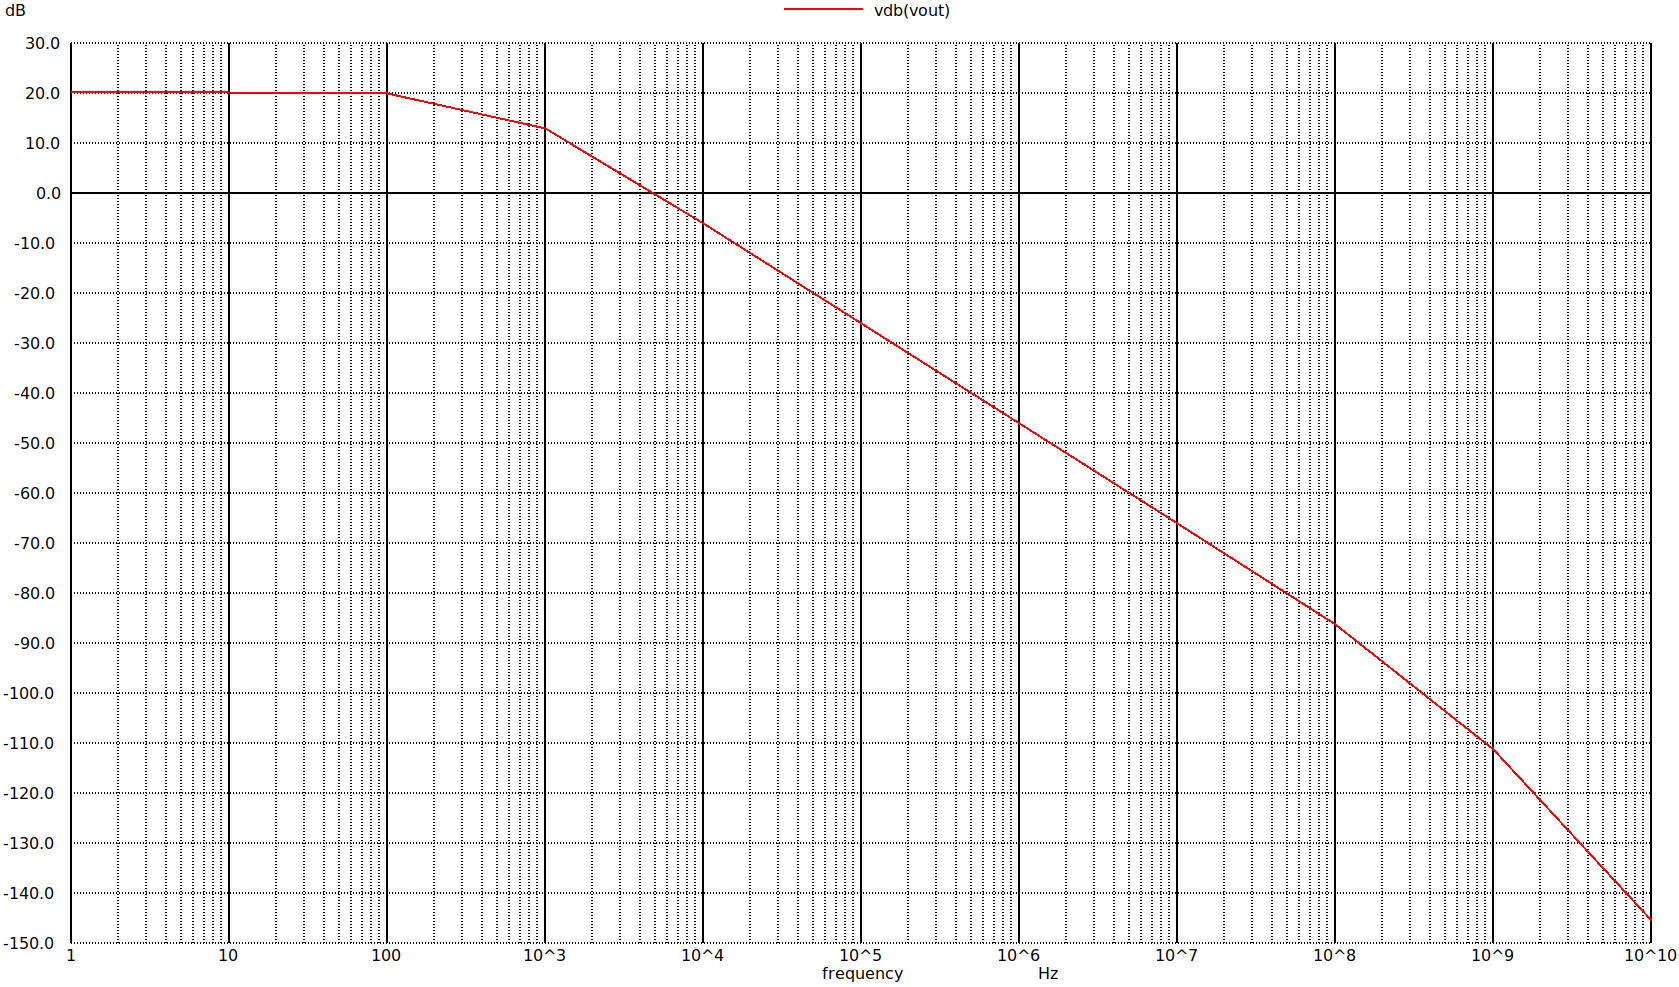
\includegraphics[scale=0.28]{CascodeOneStageOpAmpAvWF.png}
	\caption{Diagrama de Bode obtenido de la \autoref{fig:CascodeOneStageOpAmpAv}. \label{fig:CascodeOneStageOpAmpAvWF}}
\end{figure}

\begin{figure}[ht]
	\centering
	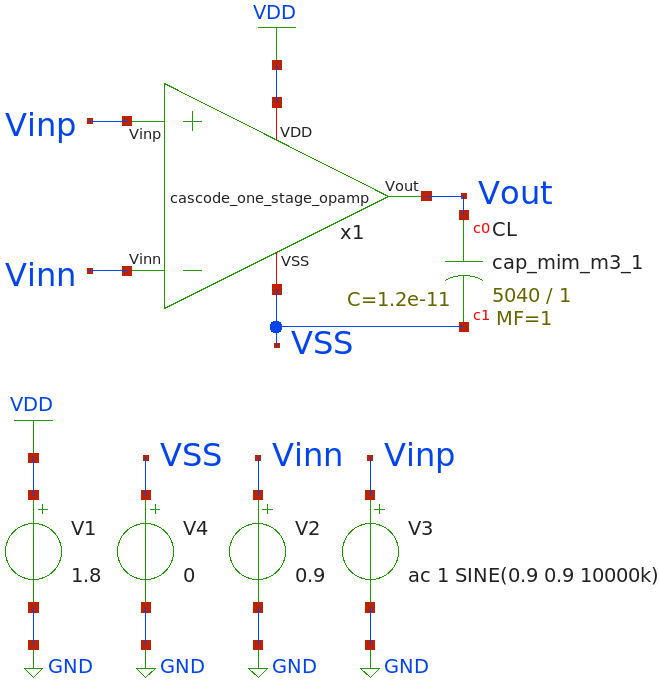
\includegraphics[scale=0.35]{CascodeOneStageOpAmpGB.png}
	\caption{Circuito utilizado para obtener la ganancia en ancho de banda (\textit{Gain Bandwidth}) del amplificador operacional cascodo de una etapa). \label{fig:CascodeOneStageOpAmpGB}}
\end{figure}

\begin{figure}[ht]
	\centering
	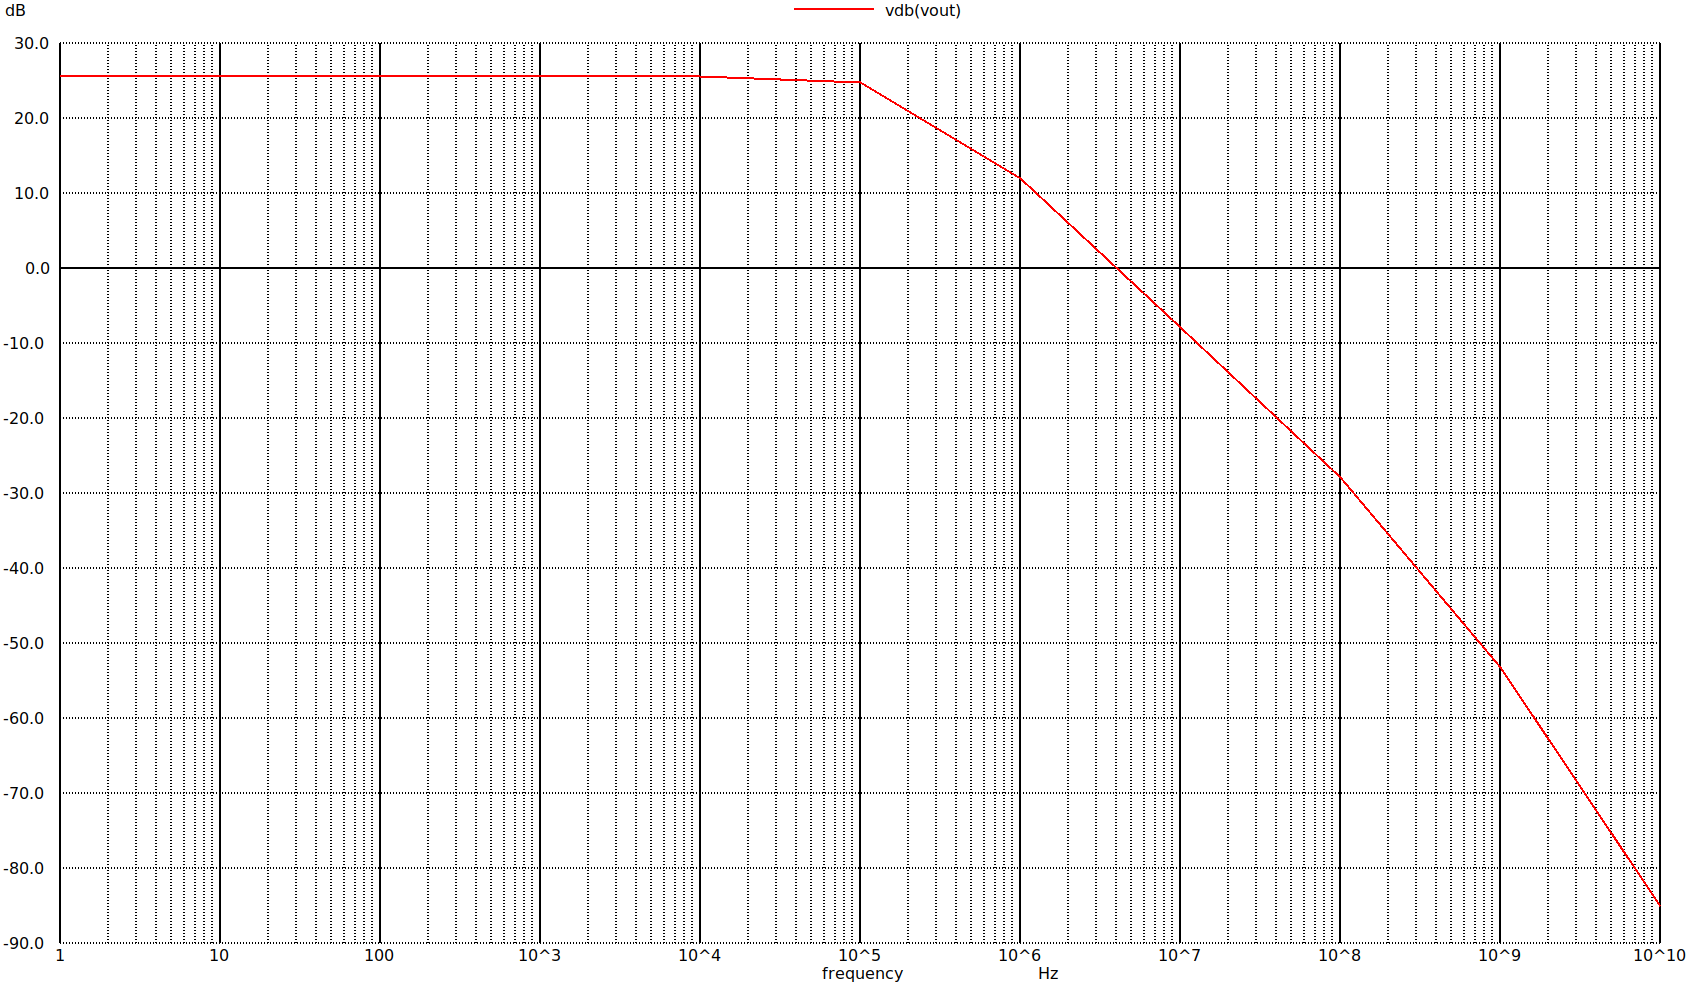
\includegraphics[scale=0.28]{CascodeOneStageOpAmpGBWF.png}
	\caption{Diagrama de Bode obtenido de la \autoref{fig:CascodeOneStageOpAmpGB}. \label{fig:CascodeOneStageOpAmpGBWF}}
\end{figure}

\begin{figure}[ht]
	\centering
	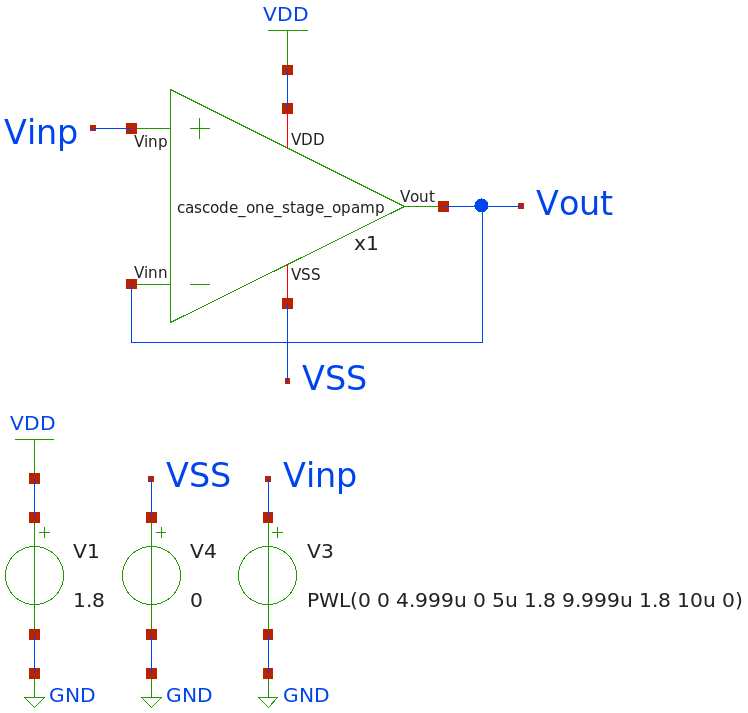
\includegraphics[scale=0.35]{CascodeOneStageOpAmpSR.png}
	\caption{Circuito utilizado para evaluar obtener el \textit{Slew Rate} del amplificador operacional cascodo de una etapa (Seguidor de voltaje). \label{fig:CascodeOneStageOpAmpSR}}
\end{figure}

\begin{figure}[ht]
	\centering
	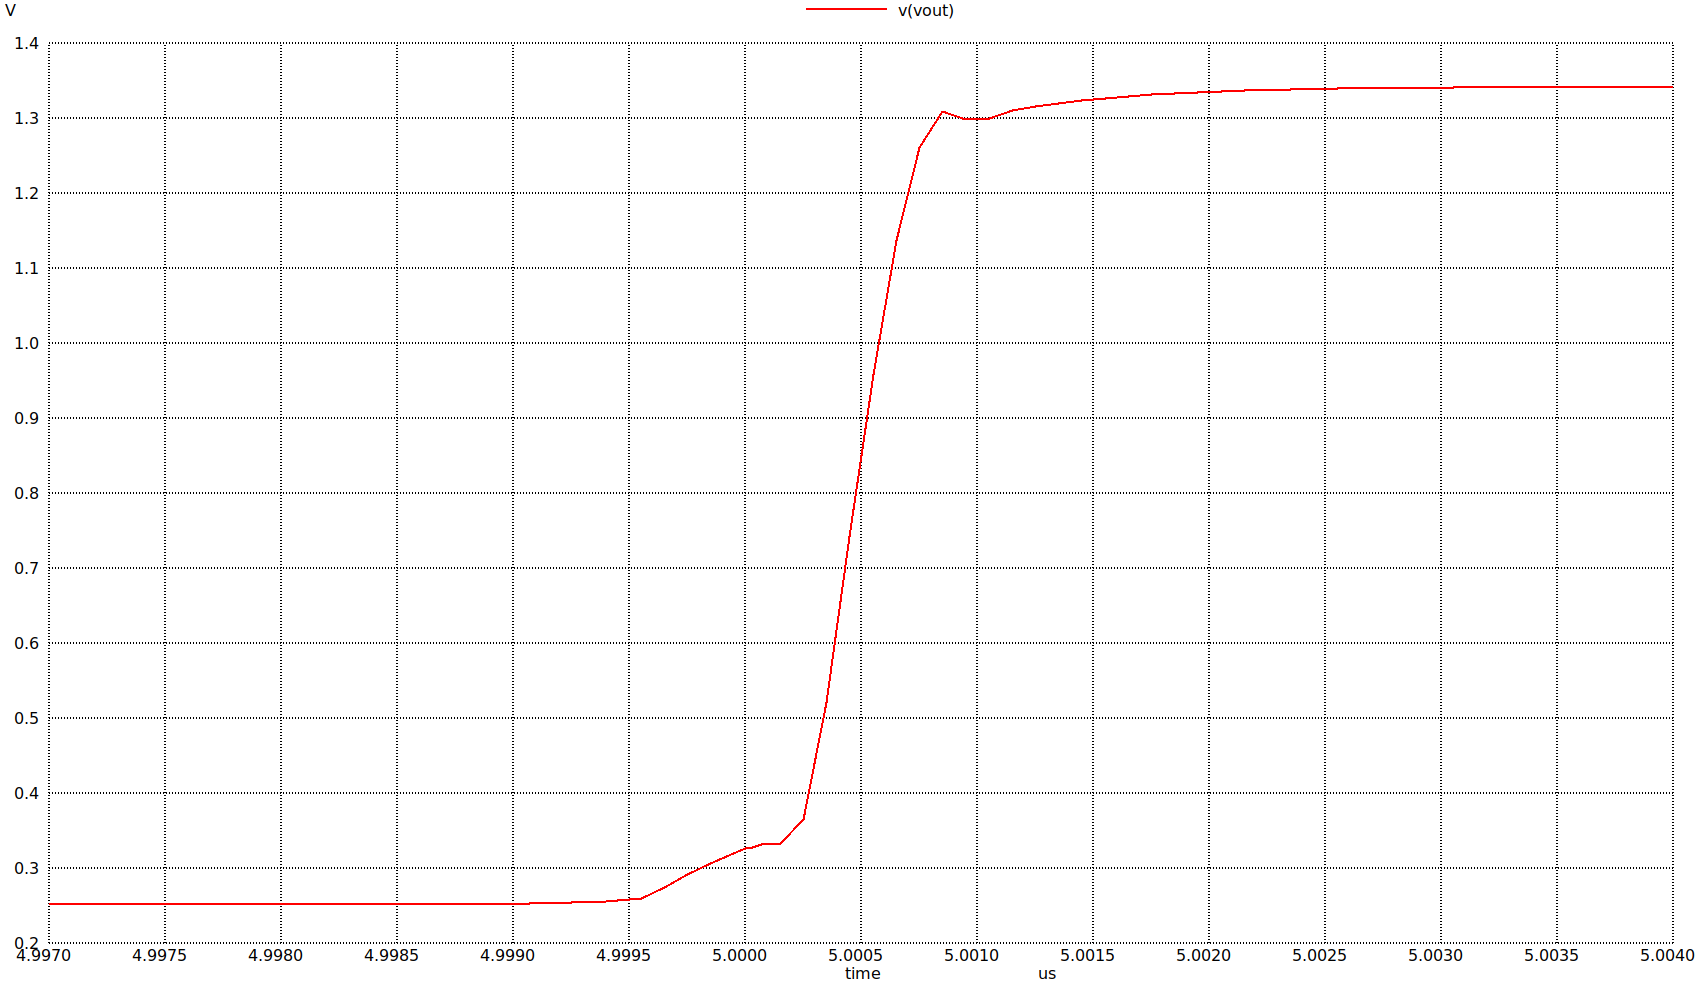
\includegraphics[scale=0.28]{CascodeOneStageOpAmpSRWF.png}
	\caption{Grafica del voltaje de salida obtenido de la \autoref{fig:CascodeOneStageOpAmpSR}. \label{fig:CascodeOneStageOpAmpSRWF}}
\end{figure}

\begin{equation*}
	\begin{array}{l l}
		\textbf{Resultados obtenidos de la simulación} \\
		A_{V} = \frac{A_{V}(0)}{R \times C} = \frac{ 15.742238 }{ 100000.0 \times 1.2e-08 } \\
		A_{V} =  131.18532  \\
		P_{diss} = V_{DD} \times I_{5} =  1.8 \times 6e-05  \\
		P_{diss} =  0.108  mW \\
		GB =  417.643781  KHz \\
		Slew Rate =  11.823621 \frac{V}{\mu s} \\
	\end{array}
\end{equation*}